% Anhang %
\chapter{Hintergrundwissen Arduino}


%%%%%%%%%%%%%%%%%%%%%%%%%%%%%%%%%%%%%%%%%%%%%%%%%%
%% Fehlersuche  %%%%%%%%%%%%%%%%%%%%%%%%%%%%%%%%%%
%%%%%%%%%%%%%%%%%%%%%%%%%%%%%%%%%%%%%%%%%%%%%%%%%%
\section{Fehlersuche}


%%%%%%%%%%%%%%%%%%%%%%%%%%%%%%%%%%%%%%%%%%%%%%%%%%
%% Analoge und digitale Signale %%%%%%%%%%%%%%%%%%
%%%%%%%%%%%%%%%%%%%%%%%%%%%%%%%%%%%%%%%%%%%%%%%%%%
\section{Analoge und digitale Signale}

Ein Analogsignal ist im Rahmen der Signaltheorie eine Form eines Signals mit stufenlosem und unterbrechungsfreiem Verlauf. Ein Analogsignal wird als glatte Funktion beschrieben und es lässt sich damit beispielsweise der zeitlich kontinuierliche Verlauf einer physikalischen Größe wie der Schalldruck in Form eines analogen Audiosignals beschreiben. Der Wertebereich eines Analogsignals wird als Dynamikumfang bezeichnet.

\margininfo{digital von lat. digitus = Finger; mit Fingern wird gezählt}

Ein Digitalsignal  ist eine spezielle Form eines Signals, welches einerseits einen abgegrenzten und gestuften Wertvorrat und zudem in der zeitlichen Abfolge nur zu bestimmten periodischen Zeitpunkten definiert ist bzw. eine Veränderung im Signalwert aufweist. Es kann aus einem Analogsignal, welches den zeitlich kontinuierlichen Verlauf einer physikalischen Größe beschreibt, durch die Quantisierung und eine Abtastung, welche zu definierten Zeitpunkten erfolgt, gebildet werden. Die digitalen Werte sind üblicherweise als Binärzahlen kodiert, so dass ihre Quantisierung in Bits angegeben wird.
\subsection{Digital Analog Wandler}


\subsubsection{Aufbau der Schaltung}

Der Aufbau der Schaltung ist in Abb. und Abb. \ref{fig:8bitDAC} zu sehen. 

In der Abb. \ref{fig:8bitDAC} sind neben dem eigentliche DAC-Wander bestehend aus den neuen $20k\Ohm$ und  sieben $10k\Ohm$ Widerständen ein Potentiometer, das  zur Verändern der Frequenz dient und ein Summer, dessen Aufgabe es ist das Signal akustischen darzustellen.   
  
\marginfigure{Anhang/Bilder/8bitDAC}{8 BIT Analog Digital Wander}{fig:8bitDAC}

\clearpage
\subsubsection{Beispiel-Sketch zum erzeugen eines sinusförmigen Spannungsverlaufes}

\begin{multicols}{2}
\begin{arduinoCode}{Beispielsketch für eine sinusförmigen Spannungsverlauf}{lst:8bitDAC}
int mPoti;

void setup()
{
  for (int i=0;i<8;i++) {
    pinMode(i, OUTPUT); (*@ \tikzmark{pinMode} @*)
  }
}

void loop() {
    mPoti = analogRead(A0);
    
    for (int i=0; i<8;i++) {
      digitalWrite(i, HIGH); 
      delayMicroseconds(mPoti);
      digitalWrite(i, LOW);
    }
 
    for (int i=6;i>0;i--) {
      digitalWrite(i, HIGH);
      delayMicroseconds(mPoti);
      digitalWrite(i, LOW);
    }  
}\end{arduinoCode}

\vfill
\columnbreak

\begin{itemize}
  \itemsep15pt
  \item[] \tikzmarkcomment{item1}{Digital PINs 0 bis 7 werden auf OUTPUT gesetzt}
\end{itemize}


\begin{tikzpicture}[remember picture,overlay]
  \path[red, thick,-] (pinMode.east) edge [out=0 , in=180] (item1);
 \end{tikzpicture}
\vfill 
\end{multicols}


%%%%%%%%%%%%%%%%%%%%%%%%%%%%%%%%%%%%%%%%%%%%%%%%
%% Arduinos Verbindung zur Aussenwelt: PINs %%%%
%%%%%%%%%%%%%%%%%%%%%%%%%%%%%%%%%%%%%%%%%%%%%%%%
\sectionExkurs{Arduino's Verbindung zur Aussenwelt: PINs}

Wie du schon weisst gibt es (neben anderen Anschlüssen) 14 digitale und 6 analoge PINs. In diesem Abschnitt erfährst du wichtiges Hintergrundwissen. Es ist wichtig, dass du diesen Abschnitt aufmerksam liest, da der Inhalt sehr wichtig für dein Verständnis für die Funktionsweise des Arduino-Boards ist. Wenn du mit dem Inhalt noch überfordert bis, kannst du auch zuerst mit Kapitel 2 anfangen, aber du solltest diesen Abschnitt unbedingt lesen und durcharbeiten. Ich habe versucht den Inhalt anhand von Beispielen und Aufgaben aufzulockern. Die Aufgaben sind der Schlüsel zum Verständnis.     

\subsection{Digitale Ein- und Ausgänge} 

Die digitalen PINs des Arduino's können entweder als Ein- oder Ausgänge konfiguriert werden. Du hast beide Arten schon kennengelernt. Im Abschnitt \ref{sec:blink} hast du den digitalen PIN 13 als OUTPUT-PIN  und im Abschnitt \ref{sec:kommunikation} den PIN 02 als INPUT-PIN benutzt.

\subsection{Der INPUT-Mode} 

Die digitalen PINs des Arduino's sind standardmäßig als Eingänge definiert. Es ist also nicht unbedingt nötig (aber trotzdem sinnvoll) sie als Eingänge mit dem Befehl \arduinocode{pinMode(pinNummer,INPUT);} zu definieren. Sinnvoll deswegen, damit deinen Sketch verständlicher wird. Die digitalen PINs haben einen sehr hohe Impedanz.
\margininfo{Impedanz: Die Fähigkeit einen elektrische Ladung lange zu speichern} Dies bedeutet, dass ein kleiner elektrischer Strom ausreicht, damit der PIN seinen Zustand wechselt. Dies kann zum Beispiel für einen kapazitiven Touch-Sensor benutzt werden.

Wenn ein PIN im INPUT-Mode nicht mit einem Sensor verbunden ist, wirkt sich die Hohe Impedanz negativ aus. Wenn du diesen PIN ausliest stellen sich zufällige Ergebnisse für den Zustand an diesem PIN ein! Es findet ein Kopplung mit der in seiner Umgebung vorhandenen Elektrizität statt. Das kann dein Pulli sein, der sich elektrostatisch aufgeladen hat, oder das Laptop. In diesem Fall spricht man davon, dass der Zustand des PINs nicht definiert ist.  

\subsubsection{Aufgabe 1: Ein Touch-Sensor}

Für diese Schaltung benötigt du einen großen Widerstand $(100k\Omega-1M\Omega)$, ein Krokodilklemmen-Kabel und ein Stück Metallfolie. Baue die Schaltung nach Abb. \ref{fig:CapSensor} auf und lade den Beispiel-Sketch aus Listing \ref{lst:CapSensor} auf deinen Arduino. Da die auf dem Arduino-Board am PIN 13 eingebaute LED von dem Projekt-Shield verdeckt wird, kannst du am PIN 13 und GND eine LED einstecken. Wenn du die Schaltung richtig aufgebaut hast, dann sollte die LED an PIN 13 leuchten. Berühre kurz die Metallfolie, dann erlischt die LED für eine Sekunde.   
\marginfigure{Kapitel1/Bilder/CapSensor}{Touchsensor}{fig:CapSensor}


\begin{multicols}{2}
\margininfo{Sollte der Touch-Senor nicht funktionieren, dann könnte es sein, dass du durch den Boden im Schulhaus elektrostatisch aufgeladen bist. Berühre einfach mit der anderen Hand das Gehäuse es USB-Anschlusses, dann sollte der Sensor funktionieren.}

\begin{arduinoCode}{Beispiel-Sketch für einen Touch-Senor}{lst:CapSensor}
const int capPin1 = 7;    (*@ \tikzmark{capPINs} @*) 
const int capPin2 = 8;    
const int ledPin =  13;   
int capState = 0;   (*@ \tikzmark{capState} @*)

void setup() {
  pinMode(ledPin, OUTPUT);  (*@ \tikzmark{pinModes} @*)
  pinMode(capPin1, INPUT);
  pinMode(capPin2, OUTPUT);
}

void loop() {
  capState = digitalRead(capPin1);(*@ \tikzmark{digitalRead} @*)
  digitalWrite(capPin2,HIGH);
  if (capState == HIGH) { (*@ \tikzmark{ifelse} @*)
    digitalWrite(ledPin, HIGH);
  }
  else {
    digitalWrite(ledPin, LOW);
    delay(1000);
  } 
}
\end{arduinoCode}
\vfill
\columnbreak

\null\vfill
\begin{itemize}
  \itemsep15pt
  \item[] \tikzmarkcomment{item1}{Definition der Sensor PINs}
  \item[] \tikzmarkcomment{item2}{Hier soll später der aktuelle Zustand von PIN 7  gespeichert werden.}
  \item[] \tikzmarkcomment{item3}{Deklaration der PINs}
  \item[] \tikzmarkcomment{item4}{Auslesen und speichern des Zustands am PIN 7.}
  \item[] \tikzmarkcomment{item5}{Reaktion auf den gespreicherten Zustand.}
\end{itemize}
\vfill \null

\begin{tikzpicture}[remember picture,overlay]
  \path[red, thick,-] (capPINs.east) edge [out=0 , in=180] (item1);
  \path[red, thick,-] (capState.east) edge [out=0 , in=180] (item2);
  \path[red, thick,-] (pinModes.east) edge [out=0 , in=180] (item3);
  \path[red, thick,-] (digitalRead.east) edge [out=0 , in=180] (item4);
  \path[red, thick,-] (ifelse.east) edge [out=0 , in=180] (item5);
\end{tikzpicture}

\end{multicols}



\subsection{INPUT-Mode und Pullup-Widerstände } 

Im Atmega-Chip sind $20 k\Omega$ Pullup-Widerstände eingebaut, auf die mit Hilfe von Software zugegriffen werden kann. Diese integrierten Pullup-Widerstände werden durch den Arduino-Befehl \arduinocode{pinMode(pinNummer,INPUT)} aktiviert. 

Durch die internen Pullup-Widerstände liegt an einem INPUT-PIN der HIGH-Zustand an. 



Wenn nun ein Sensor mit dem auf INPUT gesetzten digitalen PIN verbunden wird, sollte der andere Ausgang des Sensors mit GND verbunden werden. Im Fall eines einfachen Schalters bewirkt dies, dass wenn der Schalter geschlossen ist der Wert LOW und wenn er geöffnet ist der Wert HIGH am digitalen PIN anliegt.



Oft ist es nützlich, einen digitalen Eingang in einen bekannten Zustand zu steuern, wenn keine Eingabe vorhanden ist. Dies kann mit Hilfe eines Pullup-Widerstand ($+5\V$) oder eines Pulldown-Widerstand (GND) erreicht werden. Pull-Widerstand sollte um die $10k\Ohm$ groß sein. 

\subsubsection{Aufgabe 2}

Ziel dieser Aufgabe ist es das Verhalten eines Pullup- und Pulldown-Widerstandes zu testen. Baue die Schaltung aus Abb. \ref{fig:pull-resistors} auf. Der digitale PIN 03 wird mit einem  $10k\Ohm$-Widerstand mit $+5\V$ verbunden. Der digitale PIN 05 wird mit einem  $10k\Ohm$-Widerstand mit GND verbunden. Mit Hilfe des Sketches \ref{lst:pull-resistors} kannst du den jeweiligen Zustand auslesen. 

\begin{multicols}{2}
\begin{arduinoCode}{Pullup- und Pulldown-Widerstände}{lst:pull-resistors}
int pullDown = 3; (*@ \tikzmark{pullPINs} @*)
int pullUp = 5;

int valuePullDown = 0; (*@ \tikzmark{pinState} @*)
int valuePullUp = 0;

void setup() {
  
  Serial.begin(9600); (*@ \tikzmark{serial} @*)
  
  pinMode(pullDown, OUTPUT); (*@ \tikzmark{pinModes} @*)
  pinMode(pullUp, OUTPUT);
}

void loop() {
  
  valuePullDown = digitalRead(pullDown); (*@ \tikzmark{digitalRead} @*)
  valuePullUp = digitalRead(pullUp);
  
  Serial.print("Wert am PIN 3: ");
  Serial.println(valuePullDown);
  Serial.print("Wert am PIN 5: "); (*@ \tikzmark{printSerial} @*)
  Serial.println(valuePullUp);
  
  delay(200);     
}
\end{arduinoCode}
\vfill
\columnbreak

\null\vfill
\begin{itemize}
  \itemsep15pt
  \item[] \tikzmarkcomment{item1}{Definition der Pull-PINs}
  \item[] \tikzmarkcomment{item2}{Speichern der aktuellen Werte}

  \item[] \tikzmarkcomment{item3}{Starten der seriellen Verbindung}
  \itemsep25pt
  \item[] \tikzmarkcomment{item4}{Deklaration der PINs als OUTPUT, so dass der interne Pulldown-Widerstand nicht verbunden ist.}
  \item[] \tikzmarkcomment{item5}{Auslesen und speichern der Zustände am PIN 3 und 5.}
  \itemsep15pt
  \item[] \tikzmarkcomment{item6}{Ergebnis an PC übertragen.}
\end{itemize}
\vfill \null

\begin{tikzpicture}[remember picture,overlay]
  \path[red, thick,-] (pullPINs.east) edge [out=0 , in=180] (item1);
  \path[red, thick,-] (pinState.east) edge [out=0 , in=180] (item2);
  \path[red, thick,-] (serial.east) edge [out=0 , in=180] (item3);
  \path[red, thick,-] (pinModes.east) edge [out=0 , in=180] (item4);
  \path[red, thick,-] (digitalRead.east) edge [out=0 , in=180] (item5);
  \path[red, thick,-] (printSerial.east) edge [out=0 , in=180] (item6);
\end{tikzpicture}

\end{multicols}
\marginfigure{Kapitel1/Bilder/pull-resistors}{Pullup- und Pulldown-Widerstände}{fig:pull-resistors}

\subsection{PIN 13}

Der digitale PIN 13 ist etwas besonders, da er mit eine LED mit Vorwiderstand verbunden ist. Wenn du diesen PIN auf INPUT setzt, d.h. seinen internen $20k\Ohm$ Pull-up-Widerstand aktivierst, wird das Potenzial bei etwa $1,7\V$ anstatt der erwarteten $5\V$ liegen. Schuld an diesem Umstand ist die LED mit ihrem Vorwiderstand, die die Spannung nach unten ziehen. Das bedeutet, dass dieser PIN immer im Zustand LOW ist! Wenn du den PIN 13 als Eingang verwenden möchtest, musst du den PIN auf INPUT setzen und einen externen Pullup-Widerstand verwenden.



\subsubsection{Aufgabe 3} 
Für diese Aufgabe benötigst du nur das Arduino-Board. Verbinde den analogen PIN A0 mit dem digitalen PIN 13  (siehe Abb. \ref{fig:pin13}). Mit Hilfe des Sketches \ref{lst:pull-resistors} kannst du das Potenzial am PIN 13 messen. 

\marginfigure{Kapitel1/Bilder/pin13}{Potenzial am PIN 13 messen}{fig:pin13}

\begin{multicols}{2}
\begin{arduinoCode}{Verhalten des PINs 13}{lst:pull-resistors}
int pin13 = 13; (*@ \tikzmark{PIN} @*)

int pinPot = 0; (*@ \tikzmark{pinPot} @*)

void setup() {
  
  Serial.begin(9600); (*@ \tikzmark{serial} @*)
  
  pinMode(pin13, INPUT); (*@ \tikzmark{pinModes} @*)
  
}

void loop() {
  
  pinPot = anaolgRead(A0); (*@ \tikzmark{digitalRead} @*)
  
  Serial.print("Potenzial am PIN 13: ");
  Serial.println(pinPot/256); (*@ \tikzmark{printSerial} @*)
  
  delay(200);     
}
\end{arduinoCode}
\vfill
\columnbreak

\null\vfill
\begin{itemize}
  \itemsep15pt
  \item[] \tikzmarkcomment{item1}{Definition der Pull-PINs}
  \item[] \tikzmarkcomment{item2}{Speichern der aktuellen Werte}

  \item[] \tikzmarkcomment{item3}{Starten der seriellen Verbindung}
  \item[] \tikzmarkcomment{item4}{Deklaration der PINs}
  \item[] \tikzmarkcomment{item5}{Auslesen und speichern der Zustände am PIN 3 und 5.}
  \item[] \tikzmarkcomment{item6}{Ergebnis an PC übertragen.}
\end{itemize}
\vfill \null

\begin{tikzpicture}[remember picture,overlay]
  \path[red, thick,-] (PIN.east) edge [out=0 , in=180] (item1);
  \path[red, thick,-] (pinPot.east) edge [out=0 , in=180] (item2);
  \path[red, thick,-] (serial.east) edge [out=0 , in=180] (item3);
  \path[red, thick,-] (pinModes.east) edge [out=0 , in=180] (item4);
  \path[red, thick,-] (digitalRead.east) edge [out=0 , in=180] (item5);
  \path[red, thick,-] (printSerial.east) edge [out=0 , in=180] (item6);
\end{tikzpicture}

\end{multicols}


\subsection{Digitale PINs im OUTPUT Mode} 
Wenn ein digitaler PIN in den Modus OUTPUT gesetzt wird,
ist er in einem niederohmigen Zustand. Dies bedeutet, dass der Arduino sehr leicht kurzgeschlossen werden kann, indem man den PIN direkt mit GND verbindet. Ein digitaler PIN kann maximal bis zu $40\mA$ an Strom für  angeschlossene Geräte liefern. Die maximale Leistung ist groß genug um eine LED die meisten Sensoren zu versorgen, aber nicht groß genug um die Relais, Motoren, Magnetspulen zu betreiben. Diese Bauteile müssen dann mit Hilfe eines Transistor betrieben werden. 

Die digitalen PINs sind sehr empfindlich. Es ist immer eine gute Idee, PINs im OUTPUT Modus mit einem Wiederstand von mind. $220\Ohm$  mit GND zu verbinden.
Gerade bei LEDs sinkt der Widerstand, wenn sie leiten extrem ab. Bei langem Betrieb kann sowohl die LED als auch der digitale PIN verstört werden. 
 
\subsubsection{Aufgabe 4}

Digitale PINs im INPUT Mode liefern sehr wenig Strom, so dass eine LED nur schwach leuchtet. Sollte eine LED nur sehr schwach leuchten dann ist es wahrscheinlich, dass der Mode des PINs falsch gesetzt ist.

Versuche es selbst: Setzte dazu eine rote LED in PIN 13 und GND (schnelle Methode \ref{fig:arduino_blink_schaltung_schnell}) und lade den Sketch aus Listing \ref{lst:inoutled} auf deinen Arduino.  
\begin{multicols}{2}
\begin{arduinoCode}{PIN in input und output Mode}{lst:inoutled}
int ledPin = 13; (*@ \tikzmark{ledPIN} @*)
void setup() {  
}

void loop() {
  pinMode(ledPin, INPUT);
  digitalWrite(ledPin,HIGH); (*@ \tikzmark{input} @*)
  delay(2000);
  
  pinMode(ledPin, OUTPUT);
  digitalWrite(ledPin,HIGH); (*@ \tikzmark{output} @*)
  delay(2000);   
}
\end{arduinoCode}
\vfill
\columnbreak

\null\vfill
\begin{itemize}
  \itemsep15pt
  \item[] \tikzmarkcomment{item1}{Definition des LED-PINs}
  \item[] \tikzmarkcomment{item2}{INPUT-Mode}

  \item[] \tikzmarkcomment{item3}{OUTPUT-Mode}
\end{itemize}
\vfill \null

\begin{tikzpicture}[remember picture,overlay]
  \path[red, thick,-] (ledPIN.east) edge [out=0 , in=180] (item1);
  \path[red, thick,-] (input.east) edge [out=0 , in=180] (item2);
  \path[red, thick,-] (output.east) edge [out=0 , in=180] (item3);
\end{tikzpicture}

\end{multicols}

\subsection{Analoge Input PINs} 

Das Arduino Uno Board hat 6 analoge PINs die mit A0 bis A5 bezeichnet sind. Die Hauptfunktion der analogen PINs ist natürlich das Auslesen von analogen Sensoren. Zusätzlich haben die analogen PINs alle Funktionen der so genannten GPIO-PINs (General Purpose Input/Output), das heißt sie können als zusätzliche digitale PINs verwendet werden.

\subsubsection{Funktionsweise der analogen PINs: A/D-Wandler} 

Der ATmega-IC besitzt einen so genannten integrierte 6-Kanal-Analog-Digital-Wandler (kurz A/D-Wandler). Der A/D-Wandler hat einen Spannungsbereich von $0V$ bis $5\V$, dieser $5\V$ Potenzialunterschied wird in 1024 Teile aufgeteilt was einer Auflösung von 10-Bit ($2^{10} = 1024$) entspricht. 


\begin{table}[h]

\begin{center}

\tikzset{ 
    table/.style={
        matrix of nodes,
        row sep=-\pgflinewidth,
        column sep=-\pgflinewidth,
        nodes={
            rectangle,
            draw=black,
            align=center
        },
        minimum height=1.5em,
        text depth=0.5ex,
        text height=2ex,
        nodes in empty cells,
%%
        every even row/.style={
            nodes={fill=gray!20}
        },
        column 1/.style={
            nodes={text width=0.5\textwidth}
        },
        row 1/.style={
            nodes={
                fill=black!90,
                text=white,
                font=\bfseries
            }
        }
    }
}

\begin{tikzpicture}
\matrix (first) [table,text width=5em]
{   
  $U_{in}$ & 0 & 0.005  & 0.010 & \dots & 4.995 & 5.000 \\
  10-Bit Wert & 0 & 1 & 2 & \dots & 1022 & 1023 \\
};
 \end{tikzpicture}
\end{center}
\caption{Spannung und 10-Bit Wert }
\label{tab:spannung-10-bit}
\end{table}%

Um den Wert der gemessene Spannung auszugeben, muss der gemessene 10-Bit-Wert durch 256 geteilt werden. Dies kann mit Hilfe des Arduino-Befehles map() geschehen:

\subsubsection{Aufgabe 5}
Widerstandsmessung eines unbekannten Widerstandes. Mit Hilfe eines $1k\Ohm$-Widerstandes soll der Wert eines unbekannten Widerstandes bestimmt werden. Dazu müssen die Widerstände in Reihe geschaltet werden. Der unbekannte Widerstand kann dann mit Hilfe der Formel
\begin{eqnarray*}
  R_2 = \frac{U_2}{U_g-U_2}\,R_1
\end{eqnarray*}
berechnet werden. Mit $R_1=1k\Ohm$ und $U_g=5\V$ folgt:
\begin{eqnarray*}
  R_2 = \frac{U_2}{5\V-U_2}\cdot 1k\Ohm
\end{eqnarray*}
 

\marginfigure{Kapitel1/Bilder/widerstandMessung}{Widerstandsmessung}{fig:widerstandMessung}

\begin{multicols}{2}
\null\vfill
\begin{arduinoCode}{Messen eines unbekannten Widerstandes}{lst:widerstandMessung}
float senU = 0.0; (*@ \tikzmark{senU} @*)
float gemR = 0.0;

void setup() {  
  Serial.begin(9600); (*@ \tikzmark{serial} @*)
}

void loop() {
  senU = map(anaolgRead(A0),0,1024,0,5); (*@ \tikzmark{digitalRead} @*)
  
  gemR = senU/(5-senU)*1000;(*@ \tikzmark{rechnung} @*)
    
  Serial.print("R gemessen: ");
  Serial.println(gemR); (*@ \tikzmark{printSerial} @*)
  
  delay(200);     
}
\end{arduinoCode}
\vfill\null 
\columnbreak

\null\vfill
\begin{itemize}
  \itemsep15pt
  \item[] \tikzmarkcomment{item1}{Speichern der aktuellen Werte}

  \item[] \tikzmarkcomment{item2}{Starten der seriellen Verbindung}
  \item[] \tikzmarkcomment{item3}{Messen und umrechnen auf Spannungswert.}
  \item[] \tikzmarkcomment{item4}{Widerstand berechnen}
  \item[] \tikzmarkcomment{item5}{Ergebnis an den PC senden}
\end{itemize}
\vfill \null

\begin{tikzpicture}[remember picture,overlay]
  \path[red, thick,-] (senU.east) edge [out=0 , in=180] (item1);
  \path[red, thick,-] (serial.east) edge [out=0 , in=180] (item2);
   \path[red, thick,-] (digitalRead.east) edge [out=0 , in=180] (item3);
  \path[red, thick,-] (rechnung.east) edge [out=0 , in=180] (item4);
  \path[red, thick,-] (printSerial.east) edge [out=0 , in=180] (item5);
\end{tikzpicture}

\end{multicols}




\subsubsection{Das PIN Mapping}


Analoge PINs können auch als digitale PINs verwendet werden. Um sie von den digitalen PINs unterscheiden zu können, werden die Alias Namen A0 bis A5 verwendet. Um den analogen PIN A0 als digitalen Ausgang mit dem Wert HIGH zu definieren sind folgende Befehle nötig: 
\begin{multicols}{2}
\null\vfill
\begin{arduinoCode}{Analoger PIN wird zum digitalen PIN}{lst:analogPINdigital}
pinMode(A0, OUTPUT); (*@ \tikzmark{output} @*)
digital(A0, HIGH); (*@ \tikzmark{high} @*)
\end{arduinoCode}
\vfill\null 
\columnbreak

\null\vfill
\begin{itemize}
  \itemsep15pt
  \item[] \tikzmarkcomment{item1}{PIN A0 wird zu einem digitalen PIN}
  \item[] \tikzmarkcomment{item2}{A0 wird auf HIGH gesetzt}
\end{itemize}
\vfill \null

\begin{tikzpicture}[remember picture,overlay]
  \path[red, thick,-] (output.east) edge [out=0 , in=180] (item1);
  \path[red, thick,-] (high.east) edge [out=0 , in=180] (item2);
\end{tikzpicture}

\end{multicols}

\subsubsection{Aufgabe 6}
Ändere den Blink Sketch so ab, dass eine LED, die mit dem analogen PIN A0 verbunden ist mit einer Frequenz von einer Sekunde blinkt.

\marginfigure{Kapitel1/Bilder/digitalA0}{Analoger PIN A0 als digitaler PIN verwendet}{fig:digitalA0}

\subsubsection{pullup-Widerstände} 

Die analogen PINs besitzen ebenfalls Pullup-Widerstände. diese Pullup-Widerstände können mit den folgender Befehl aktiviert werden: 
\begin{arduinoCode}{}{}
digital(A0, HIGH); // Set Pullup auf analogen PIN 0 
\end{arduinoCode}
Der PIN sollte natürlich dann im INPUT-Mode sein. 

Das Einschalten des Pullup-Widerstandes verfälscht natürlich die Werte von analogRead()!

\subsubsection{Für Experten!} 

Wenn du die analogen PINs verwenden möchtest, kann es vorkommen, dass sie sich manchmal komisch verhalten.
\begin{itemize}
  \item Wenn ein analoger PIN als Ausgang definiert wurde, wird der Befehl analogRead() nicht korrekt funktionieren. Wenn dies der Fall ist, muss der PIN zuvor als Eingang definiert werden, erst dann kann der Befehl analogRead() korrekt ausgeführt werden. 
 \item  Wenn zwischen verschiedenen analogen Eingang zu schnell gewechselt wird, kann es passieren, dass  A/D-Messwerte durch elektrische Störsignale (genannt Noise) verfälscht werden. Deshalb ist es sinnvoll beim Wechseln von analogen Eingängen eine kurze Pause einzubauen.
\end{itemize}




%%%%%%%%%%%%%%%%%%%%%%%%%%%%%%%%%%%%%%%%%%%%%%%%%%
%% Interruptsteuerung %%%%%%%%%%%%%%%%%%%%%%%%%%%%
%%%%%%%%%%%%%%%%%%%%%%%%%%%%%%%%%%%%%%%%%%%%%%%%%%

\section{Interruptsteuerung}
 
Der Mikrocontroller des Arduino ist mit einer Interrupt-Steuerung (IRC) ausgestattet. Die Aufgabe einer IRC ist es auf stattfindende Ereignisse sofort zu reagieren. Dazu wird die aktuelle Aufgabe unterbrochen und sofort auf das Ereignis zu reagieren.
Man könnten Sie sich fragen, warum ein Interrupt notwendig ist,  um auf externe Ereignisse zu reagieren?
Schließlich können man den Zustand  externer Pins jederzeit überprüfen.

Das Problem ist, dass wenn die Aufgaben komplexer werden, es sicherlich nicht sinnvoll ist alle Abläufe 
in der Loop-Routine abzuarbeiten. Das auf bestimmte Signale unterbrechen der Loop-Routine ist ein
entscheidenden Vorteil - die Unterbrechungen  sind asynchron. 

Ein asynchrones Ereignis ist etwas, das außerhalb des regulären Ablauf der Loop-Routine auftritt -- es
kann jederzeit passieren, egal, was Ihr Sketch im Moment gerade ausführt. Dies bedeutet, dass anstatt 
manuell prüfen, ob ein bestimmtes  Ereignis eintritt, übernimmt diese Aufgabe der Mikrocontroller selbst.

Wenn ein Projekt  ein  genaues Timing verlangt oder schnell auf Eingaben (z.B. von Sensoren) 
reagieren soll,  dann sind Interrupts das Mittel der Wahl. Im folgenden Abschnitt erkläre ich die 
Funktion und Verwendung von Interupts. \citet{engblaze_we_2013}


%Lassen Sie uns ein Beispiel aus der Praxis. Stell dir vor du bist auf der Couch sitzen, genießen einen frostigen brauen und einen Film nach einem langen Tag. Das Leben ist gut. Es gibt nur ein Problem: Sie suchen nach einem unglaublich wichtiges Paket zu kommen warten, und Sie müssen sie so bald wie möglich. Wenn Sie einen normalen AVR-Programm oder Arduino Sketch waren, man müsste wiederholt stilllegen Ihren Film, aufstehen und gehen überprüfen Sie die Mailbox alle 5 Minuten, um sicherzustellen, dass Sie wissen, wann das Paket da war.
%
%Stattdessen vorstellen, wenn das Paket Fedex oder UPS mit Lieferbestätigung versendet. Nun wird die Lieferung Mann bis vor die Haustür und Ring gehen die Türklingel, sobald er ankommt. Das ist Ihre Interrupt auslösen. Sobald Sie den Auslöser, können Sie Pause Ihren Film und gehen viel mit dem Paket. Das ist Ihre Interrupt-Service-Routine. Sobald Sie fertig sind, können Sie abholen den Film wo Sie aufgehört haben, ohne zusätzliche Zeit verschwendet. Das ist die Macht von Interrupts.
%
%Die AVR-Chips in den meisten Arduinos verwendet werden, sind nicht in der Lage parallele Verarbeitung, dh sie können nicht mehrere Dinge auf einmal. Mit asynchrone Verarbeitung über Interrupts ermöglicht es uns, die Effizienz unseres Codes zu maximieren, so dass wir nicht verschwenden keine kostbare Takte am Abfrageschleifen oder warten auf Dinge geschehen. Interrupts sind auch gut für Anwendungen, die präzises Timing erfordern, weil wir wissen, wir fangen unsere Veranstaltung, sobald es auftritt, und nicht versehentlich verpassen.


\subsection{Was sind Interrupts?}

Im Grunde ist ein Interrupt ein Signal, das den ablaufenden Prozess unterbricht. Dieses Signal 
kann entweder durch ein externes Ereignis (z.B. die Änderung eines digitalen Pin Zustandes) oder durch 
ein internes Ereignis (z.B. ein Zeitsignal eines Softwaretimers) ausgelöst werden.

Einmal ausgelöste (triggered), wird ein Interrupt den zur Zeit ablaufenden Prozess anhalten (den 
Zustand dieses Prozesses speichern)  und eine so genannte ``interrupt service routine'' (ISR) 
ausführen. Die ISR reagiert auf den Interrupt, wenn die Abgeschlossen ist, wird er zuvor aufgeführte 
Prozess fortgeführt. 

\begin{figure}[ht]
\begin{center}

% Define a few styles and constants
\tikzstyle{hp}=[draw, fill=blue!20, text width=8em, rounded corners,
    text centered, minimum height=2.5em]
\tikzstyle{irq1} = [hp, fill=red!20]
 
\tikzstyle{pfeil}=[draw,->,black!80,thick,double]
    
\def\blockdist{3.3}
\def\edgedist{2.5}

\begin{tikzpicture}
   \draw[->,thick] (-2,-1) -- (12,-1) node[below=1mm,midway,text width=3cm,text centered] {time};
   \draw[-, thick] (1.7,-1.2) -- (1.7,-0.8)  node[below=1mm,midway,text width=3cm,text centered] {IRQ Signal};
   
   \node (hp1) at (0,0) [hp] {Hauptprozess}; 
   \node (irq) at (5,2.5) [irq1]  {ISR-Routine};  
   \node (hp2) at  (10,0) [hp] {Hauptprozess};
 
    \draw [-to,thick,snake=snake,segment amplitude=.8mm,
         segment length=5mm,line after snake=1mm]
    (hp1.east) -- (irq.west) node [midway] {HP wird unterbrochen};
    \draw [-to,thick,snake=snake,segment amplitude=.8mm,
         segment length=5mm,line after snake=1mm]
    (irq.east) -- (hp2.west) node [midway] {HP wird fortgesetzt};
\end{tikzpicture}
 
\caption{Funktionsweise eines IRQs, das Hauptprogramm wird unterbrochen um die IRQ-Routine auszuführen.}
\label{fig:irq}
\end{center}
\end{figure}



\subsubsection{Die verschiedenen Arten von Interrupts}
Es gibt im Wesentlichen zwei Arten von Interrupts:
\begin{itemize}
\item Hardware-Interrupts, die auf ein externes Ereignis reagieren, wie z. B. wenn bei einem Eingangspin 
der logische Zustand von HIGH nach LOW wechselt.
\item Software-Interrupts, die  auf eine Software Ereignis reagieren.
\end{itemize}
Die 8-bit AVR-Prozessoren,  die meistens in Arduino-Boards verbaut sind, sind  nicht in der Lage auf 
Software-Interrupts zu reagieren.

In  der  Arduino-Sprache  gibt es deshalb nur eine einzige Art von 
Interrupts, die attachInterrupt()-Funktion. 

Für einfache Anwendungen ist diese Funktion ausreichend, aber es gibt noch eine ganz andere Art von
Hardware-Interrupts. 

\subsection{Die Interrupt Service Routines}


Jeder Prozessor AVR hat eine Liste von Interrupt-Quellen, oder Vektoren, die die Art der Ereignisse, die 
einen Alarm auslösen können, umfassen. 
Die Interrupt-Vektor - wenn Interrupts aktiviert sind und eines dieser Ereignisse eintritt, wird der Code an
einer bestimmten Stelle im Programmspeicher springen. Durch das Schreiben eines ISR und dann die 
Anbringung eines Links die es bei der Interrupt-Vektors Speicherplatz, können wir sagen unseren Code, 
um etwas Bestimmtes, wenn ein Alarm ausgelöst wird tun.

Implementieren wir dies mit einem einfachen Beispiel: Erkennen, wann eine Taste gedrückt wurde, und 
eine Aktion auf diesem Pressefreiheit. In diesem Tutorial verwenden wir ein Standard Arduino-Board, um 
die Dinge konsequent, wenn wir uns auf die Pins und unser Programm Setup beziehen. Sie können 
diese Techniken mit einem einfachen AVR zu nutzen, brauchen Sie nur auf das Datenblatt überprüfen, 
um sicherzustellen, dass Sie wissen, welche Pins die Sie benötigen. Hier ist unser Beispiel Schaltung:

\subsubsection{Die Arduino Interrupt-Funktion}

\subsubsection{Implementierung eines Interrupt in einem  Sketch}


%\subsection{AVR und Arduino timer interrupts}
%
%\subsubsection{Was ist ein timer?}
%\subsubsection{Wie arbeiten timer?}
%\subsubsection{Verschiedene Arten von timers}
%\subsubsection{Konfiguration und Ausführen eines timers}
%\subsubsection{Timer prescaling and CTC}



\chapter{Data Kommunikations Systeme}
%%%%%%%%%%%%%%%%%%%%%%%%%%%%%%%%%%%%%%%%%%%%%%%%%%
%% Serielle Schnittstelle %%%%%%%%%%%%%%%%%%%%%%%%
%%%%%%%%%%%%%%%%%%%%%%%%%%%%%%%%%%%%%%%%%%%%%%%%%%
\section{Serielle Schnittstelle - die Verbindung mit dem PC}

Die verschiedenen Komponenten eines Computersystems müssen Informationen austauschen, dieser Austausch vollzieht sich mit Hilfe von Schnittstellen. Es macht sinn, für diese Schnittstellen bestimmte Konventionen festzulegen und einzuhalten, damit die Datenkommunikation reibungslos ablaufen kann. Eine mögliche Schnittstelle ist die sog. serieller Schnittstelle.

\subsection{Die TTY-Schnittstelle} 
Die TTY-Schnittstelle ist die älteste serielle Schnittstelle und wurde ursprünglich zur Verbindung von Fernschreibern entwickelt.  Da im Ruhezustand ein konstanter Gleichstrom von 20 mA fließt, wird die Schnittstelle oft auch als 20-mA-Stromschnittstelle bezeichnet.
\margininfo{Der Optokoppler dient zur galvanische Trennung von Sender- und Empfänger-Stromkreis.}
\begin{figure}[htbp]
  \begin{center}
  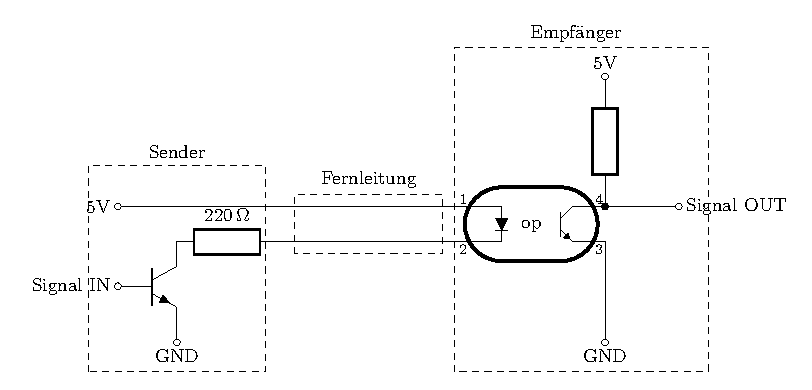
\includegraphics[width=0.8\textwidth]{Anhang/Tikz/tty-schaltung.pdf}
  \caption{TTY Schaltung (nur eine Richtung)}
  \label{fig:ttySchaltung}  
  \end{center}
\end{figure}
Die Übertragung von Daten geschieht nun einfach so, dass der Sender den Schleifenstrom in einem bestimmten Rhythmus unterbricht. Der Empfänger erkennt die rhythmischen Unterbrechungen. Für diese Art der Datenübertragung genügt eine 2-adrigen Leitung ohne. Die Datenübertragung funktioniert aber immer nur ein eine Richtung. Für den gleichzeitigen Datenversand benötigt man getrennte Stromschleifen für Senden und Empfang. Heute wird die TTY-Schnittstelle mit moderne Halbleiterbauelemente realisiert. Der Strom wird mit Hilfe eines Schalttransistor modelliert, der Empfang der Daten durch einen Optokoppler (siehe Abb. \ref{fig:ttySchaltung}).

\subsection{Aufbau eines seriellen Datenpakets}
Auf der Leitung liegt zu jedem Zeitpunkt nur ein BIT (siehe Abb. \ref{fig:serialDaten}). 
Die zu übertragende Daten werden in einzelnen Datenpakete aufgeteilt. Ein Datenpaket besteht aus 7-Daten-BITs und 3 Steuerung-BITs.

\begin{figure}[htbp]
  \begin{center}
      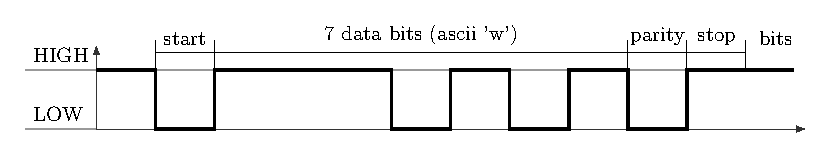
\includegraphics{Anhang/Tikz/serialDaten.pdf}
  \end{center}
  \label{fig:serialDaten}
  \caption{Serielles Datenpaket (das 7-BIT ASCII-Zeichen 'w' wird übertragen)}
\end{figure}

Jedes Datenpaket beginnt mit dem start-BIT (log. LOW). Danach folgen die chrakter-BITs die zu sendenden Daten (z.B. sieben Bit des ASCII-Codes). Als Abschluss folgt das paritäts-BIT und ein oder zwei stop-BITs (log. HIGH), worauf die Leitung wieder im Ruhezustand (log. HIGH) ist. 

Jedes BIT liegt für die gleiche, feste Zeitspanne auf der Leitung. Die Übertragungsgeschwindigkeit wird in Boud angegeben. \margininfo{Die Firma Baudot, eine Pionier der Fernschreibertechnik war Namensgeber für die Einheit Boud \\ 1 Baud = 1 Bit pro Sekunde.} 
Denn zwischen einzelnen Datenpaketen die Leitung beliebig lange im Ruhezustand verharren kann, ist die maximale Übertragungsgeschwindigkeit erreicht, wenn die Datenpakete, direkt aufeinaderfolgen. Wenn zum Beispiel einzelne 7-Bit-ASCII-Zeichen übertragen werden, so ergibt sich bei 9600 Baud eine maximale Datenrate von $ 9600/(7+3) = 960 $ Zeichen pro Sekunde. 

Damit der Empfänger ein Datenpaket empfangen kann muss er zum einen den Anfang und das Ende des Datenpakets erkennen. Zusätzlich zu den Datenbits kann ein sog. Paritäts-BIT übertragen werden mit dessen Hilfe der  Empfänger Übertragungsfehler erkennen kann.  

\subsubsection{start-BIT}
Jeden Datenpaket wird durch das Start BIT eingeleitet. Werden keine Daten übertragen, befindet sich die Leitung im Ruhezustand (log. HIGH). Das Start BIT setzt die Leitung für die Dauer eines BITs auf log. LOW. Der Empfänder weiss nun, dass die folgenden 7 BITs die Daten enthalten.


\subsubsection{parity-BIT}
Das Parität BIT ermöglicht eine primitive Fehlerkontrolle. Wird mit gerader Parität gearbeitet, so setzt der Sender das Paritätsbit auf log. HIGH, falls die Daten-BITs eine ungerade Anzahl von gesetzten (log. HIGH) BITs enthält. Bei einer geraden Anzahl wird das Paritätsbit auf log. LOW gesetzt. Der Empfänger prüft nun nach der gleichen Vorschrift, ob das Paritätsbit zu den Datenbits 'passt'. Falls bei der Übertragung eines der Datenbits verfälscht worden ist, so ist dies also vom Empfänger erkennbar. Wenn zwei Übertragungsfehler vorliegen, dann kann der Empfänger das nicht mehr erkenne.


\subsubsection{stop-BIT}

Das stop-BIT (log. LOW) beendet das Datenpaket. Danach geht die Datenleitung in den Ruhezustand (log. HIGH) über. Dieser Ruhezustand besteht bis zum nächsten Start BIT   


\subsection{RS-232: eine moderne serielle Schnittstelle}
Die RS-232-Schnittstelle wurde ursprünglich bei Großcomputern verwendet, um Terminals an einen Zentralrechner anzuschließen. 
 \marginfigure{Anhang/Tikz/serial-schnittstellen.pdf}{tx und rx PINs auf dem Arduino Board}{fig:serial-schnittstellen}
Sie wurde bis zur Einführung der USB-Schnittstelle auch zum Anschluß von Peripheriegeräten (zum Drucker, Modem etc) an einen Rechner benutzt. Bei technischen Anwendungen, wie zum Beispiel CNC-Maschinen wird die serielle Schnittstelle heute immer noch verwendet. Physikalisch ist die RS-232-Schnittstelle eine Spannungsschnittstelle für jede Richtung ist eine Signalader erforderlich, dazu kommt eine gemeinsame GND-Leitung. \margininfo{Der PIN zum Senden von Daten wird tx (transmit) und zum empfangen von Daten rx (recieve) genannt.} 


\subsection{UART serieller Interface-IC}
Prinzipiell kann man das serielle Datenpaket softwaretechnisch erzeugen, indem man eine digitalen PIN  zu den richtigen Zeitpunkten auf LOW oder HIGH setzt. Der Datenempfang per Software ist schon etwas schwieriger zu bewältigen. In der Praxis verwendet man meist einen seriellen Interface-IC, UART \margininfo{UART steht für Universal Asynchronous Receiver and Transmitter}  genannt. Das Arduino Board besitzt einen UART-Port, dieser kann mit Hilfe der System-Bibliothek Serial gesteuert werden. 

\subsection{Softwaretechnisch Daten von Arduino zu Arduino senden}
Obwohl es für das senden von Daten über eine serielle Schnittstelle die Systembibliothek Serial gibt, mach es Sinn sich die ganze Sache genauer anzuschauen und selber eine Softwarelösung zu programmieren.
 
\subsubsection{Aufbau der Schaltung}
Für den Aufbau einer seriellen Verbindung unter zwei Arduinos müssen nur zwei digtiale PINs und zwei GND PINs miteinander verbunden werden.
\begin{figure}[h]
  \begin{center}
    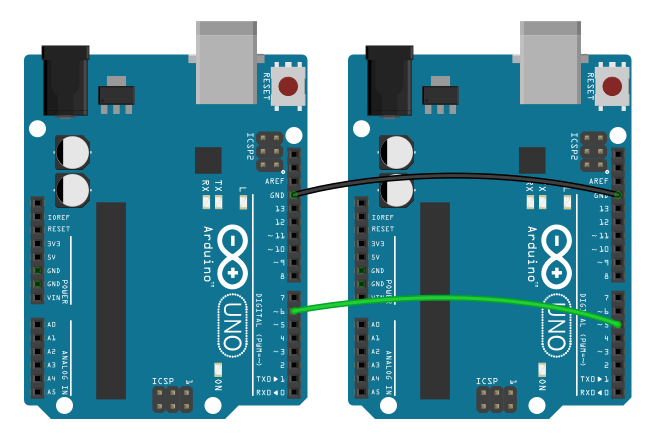
\includegraphics[width=0.6\textwidth]{Anhang/Bilder/arduino-to-arduino.png}
  \end{center}
  \label{fig:arduino-to-arduino}
  \caption{Arduino zu Arduino Verbindung mit einer seriellen Schnittstelle}
\end{figure}
  
\subsubsection{Das Senden von Daten}

\begin{multicols}{2}
\begin{arduinoCode}{}{}
#include <ctype.h>
#define bit9600Delay 84 (*@ \tikzmark{delay} @*)  

byte tx = 6;

void setup() {
  pinMode(tx,OUTPUT);
  digitalWrite(tx,HIGH);
}

void SWprint(int data)
{
  byte mask;
  digitalWrite(tx,LOW); (*@ \tikzmark{startBit} @*)
  delayMicroseconds(bit9600Delay); 
  for (mask = 0x01; mask>0; mask <<= 1) {
    if (data & mask){ // choose bit
     digitalWrite(tx,HIGH); (*@ \tikzmark{highBit} @*)
    }
    else{
     digitalWrite(tx,LOW); (*@ \tikzmark{lowBit} @*)
    }
    delayMicroseconds(bit9600Delay);
  }
  digitalWrite(tx, HIGH); (*@ \tikzmark{stopBit} @*)
  delayMicroseconds(bit9600Delay);  
 
}

void loop()
{
    SWprint(toupper('w'));      
}
\end{arduinoCode}

\vfill
\columnbreak

\begin{itemize}
  \itemsep15pt
  \item[] \tikzmarkcomment{item1}{Initialisieren der Schleifenvariablen}
\end{itemize}


\begin{tikzpicture}[remember picture,overlay]
  \path[red, thick,-] (delay.east) edge [out=0 , in=180] (item1);
 \end{tikzpicture}
\vfill 
\end{multicols}

\subsubsection{Das Empfangen von Daten}

\begin{multicols}{2}
\begin{arduinoCode}{}{}
#include <ctype.h>
#define bit9600Delay 84 (*@ \tikzmark{delay} @*)  

byte rx = 5;
byte SWval;

void setup() {
  pinMode(rx,INPUT);
}

int SWread() {
  byte val = 0;
  while (digitalRead(rx));
  if (digitalRead(rx) == LOW) {
    delayMicroseconds(halfBit9600Delay);
    for (int offset = 0; offset < 8; offset++) {
     delayMicroseconds(bit9600Delay);
     val |= digitalRead(rx) << offset;
    }
    delayMicroseconds(bit9600Delay); 
    delayMicroseconds(bit9600Delay);
    return val;
  }
}

void loop()
{
    SWval = SWread(); 
}
\end{arduinoCode}

\vfill
\columnbreak

\begin{itemize}
  \itemsep15pt
  \item[] \tikzmarkcomment{item1}{Initialisieren der Schleifenvariablen}
\end{itemize}


\begin{tikzpicture}[remember picture,overlay]
  \path[red, thick,-] (delay.east) edge [out=0 , in=180] (item1);
 \end{tikzpicture}
\vfill 
\end{multicols}

\subsubsection{Ergebnis}

\begin{figure}[htbp]
  \begin{center}
    \subfigure[]{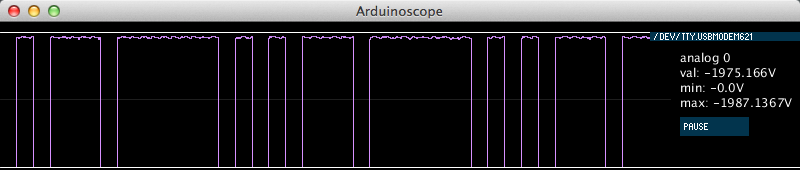
\includegraphics[width=0.7\textwidth]{Anhang/Bilder/serialW.png}}
    \subfigure[]{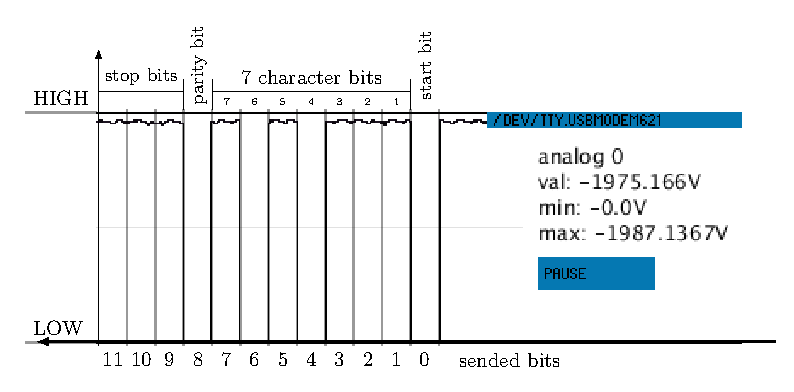
\includegraphics[width=0.6\textwidth]{Anhang/Tikz/serial-wo.pdf}}
  \end{center}
  \label{fig:serialW}
  \caption{Serielles Signal}
\end{figure}

\section{I2C Schnittstelle}

Der I2C Bus ist ein synchroner serieller 2-Draht Bus, der in den 80er Jahren von Philips entwickelt wurde. I2C gesprochen 'I Quadrat C' kommt von der der Abkürzung IIC und bedeutet Inter-Integrated Circuit. Er wird hauptsachlich dazu benutzt, zwischen Schaltkreisen, die sich auf einer Platine verbinden, Daten auszutauschen. Die beiden Leitungen, die den I2C Bus bilden heißen SCL und SDA. SCL steht für Signal Clock und ist die Taktleitung für den Bus. Deshalb spricht man auch von einem synchronen Bus. SDA steht für Signal Data und ist die Datenleitung. Die Datenübertragungsrate des I2C Busses beträgt 100kHz im Standard Mode, bzw. 400kHz im Fast Mode. Aus Lizenzgründen nennt man das I2C Interface bei Atmel TWI (Two Wire Interface).

Der I2C Bus ist ein Multi Master/Slave Bus. Das bedeutet, es gibt mindestens einen I2C Master und ebenso mindestens einen I2C Slave. Der Master selektiert einen Slave durch seine Slave Adresse, die innerhalb eines Busses eindeutig sein muss. Eine Datenübertragung kann nur durch einen I2C Master initiiert werden. Der Slave bleibt immer passiv und lauscht nur auf die Slave Adresse und vergleicht diese mit seiner eigenen Slave Adresse. Erst wenn er seine Slave Adresse erkennt, greift der Slave auch aktiv in das Busgeschehen ein.

Aus Sicht des I2C Masters unterscheidet man zwischen Read und Write Sequenzen. Bei einer Read Sequenz liest der I2C Master Daten vom I2C Slave. Bei einer Write Sequenz sendet der I2C Master Daten zum Slave.



\chapter{Hintergrundwissen: Programmieren}

\section{Rechnen im dem Mikrocontroller}

\section{Programmablaufplan }

\chapter{Hintergrundwissen: Elektronik} \label{ch:anhang_elektronik}

\section{Multimeter}

\begin{multicols}{2}
\begin{tikzpicture}
  % grid 
  \draw[color=red,help lines,xstep=1,ystep=1] (0,0) grid (6,10);
  \draw[help lines,thin,xstep=.5,ystep=.5] (0,0) grid (7,10);
  \foreach \x in {0,1,...,7} { \node [anchor=north] at (\x,0) {\x}; }
  \foreach \y in {0,1,...,10} { \node [anchor=east] at (0,\y) {\y}; }
  % Image
  \node[anchor=south west,inner sep=0] (image) at (0,0) {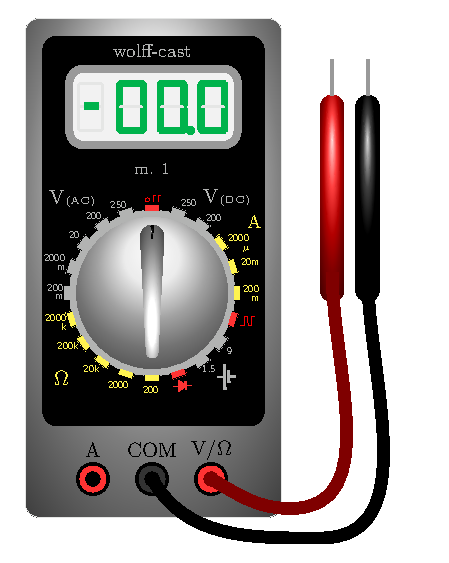
\includegraphics{Anhang/Tikz/multimeter.pdf}};
  % Marks 
  \node[] at (4,8) {\tikzmark{lcd}};
  \node[] at (2.8,4) {\tikzmark{wire}};
  \node[] at (2.05,3.4) {\tikzmark{crystal}};
  \node[] at (2.6,0.5) {\tikzmark{anode}};
  \node[] at (1.4,-0.5) {\tikzmark{cathode}};
  cathode
\end{tikzpicture}

\columnbreak
\vfill\null 
\begin{itemize}
  \itemsep20pt
    \item[] \tikzmarkcomment{item1}{4 stellige LCD-Anzeige}
    \item[] \tikzmarkcomment{item2}{Anschlussdraht für den Halbleiterkristall aus Gold}
    \item[] \tikzmarkcomment{item3}{Halbleiterkristall in Reflektorwanne}
    \item[] \tikzmarkcomment{item4}{Anode der LED (Langer PIN)}
    \item[] \tikzmarkcomment{item5}{Kathode der LED (Kurzer PIN)}
 \end{itemize}
\vfill \null

\begin{tikzpicture}[remember picture,overlay]
  \path[red, thick,-] (lcd.east) edge [out=0 , in=180] (item1);
  \path[red, thick,-] (wire.east) edge [out=0 , in=180] (item2);
  \path[red, thick,-] (crystal.east) edge [out=0 , in=180] (item3);
  \path[red, thick,-] (anode.east) edge [out=0 , in=180] (item4);
  \path[red, thick,-] (cathode.east) edge [out=0 , in=180] (item5);
\end{tikzpicture}
\end{multicols}


\section{Farbcodes von Widerständen} 

Auf Schichtwiderstände  werden die Widerstandswerte  mit Hilfe von farbigen Ringen aufgemalt. Dies hat gegen¸ber Aufschriften den Vorteil, dass die Kennzeichnung eines in eine Schaltung eingelˆteten Widerstandes auf jeden Fall zu erkennen ist. Um den Widerstandswert bestimmen zu kˆnnen, braucht man den Farbcode. Bei einem Widerstand mit vier Ringen geben die ersten beiden Ringe die Zahlen vor der Zehnerpotenz an. Die Farbe des dritten Rings gibt den Exponenten der Zehnerpotenz an. Der vierte, etwas abgesetzte Ring macht eine Angabe ¸ber die Toleranz des Widerstandswertes. Fehlt der Toleranzring, so kann man davon ausgehen, dass der Widerstandswert nur auf $\pm20\%$ genau ist.
\begin{table}[h]

\begin{center}
\begin{tabular}{|p{0.2\textwidth}|c|c|c|c|}\hline 
\rowcolor{lightgray} Ringfarbe      & \multicolumn{4}{c|}{Ring Nr. 1 -- 4 } \\\hline 
Silber  \cellcolor{silver}    & -- & -- & $10^{-2}$  &  $\pm10$\%\\\hline
Gold    \cellcolor{gold}    & -- & -- &  $10^{-1}$ &  $\pm5$\%\\\hline
\textcolor{white}{Schwarz}  \cellcolor{black}& -- & 0 & $10^{0}$   &  --  \\\hline
Braun   \cellcolor{brown}   & 1 & 1 & $10$            &  $\pm1$\%\\\hline
Rot    \cellcolor{red}      & 2 & 2 & $10^{2}$    &  $\pm2$\%\\\hline
Orange   \cellcolor{orange}& 3 & 3 & $10^{3}$    &  --\\\hline
Gelb      \cellcolor{yellow} & 4  & 4 & $10^{4}$ &  \\\hline
Gr¸n      \cellcolor{green} & 5  & 5 & $10^{5}$ &  $\pm0.5$\%\\\hline
Blau       \cellcolor{blue} & 6  & 6 & $10^{6}$ &  $\pm0.25$\%\\\hline
Lila         \cellcolor{violet} & 7  & 7 & $10^{7}$ &  $\pm0.1$\%\\\hline
Grau        \cellcolor{gray}  & 8  & 8 & --              &  $\pm0.05$\%\\\hline
Weiß       & 9  & 9 & --              &  -- \\\hline
\end{tabular}
\end{center}
\caption{Farbkodes von Kohleschichtwiderständen}
\label{tab:farbcodes}
\end{table}%

\textbf{Aufgabe:} Bestimme die Widerstandswerte folgender Widerstände. \\[0.2cm]
\begin{minipage}{0.3\textwidth}
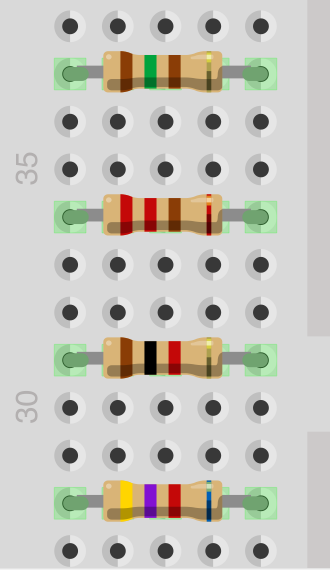
\includegraphics[width=0.8\textwidth]{Anhang/Bilder/widerstaede}
\end{minipage}
\begin{minipage}{0.7\textwidth}
\begin{itemize}
\item[a)] 
\begin{tabular}{|p{0.15\textwidth}|p{0.1\textwidth}|p{0.1\textwidth}|p{0.1\textwidth}|p{0.1\textwidth}|p{0.2\textwidth}|}\hline 
\rowcolor{lightgray} Ring Nr.      & 1 & 2 & 3 & 4  & Ergebnis \\\hline 
Farbe   & braun & rot &  braun & gold & -- \\\hline
Wert     &  1        & 5    & $\cdot 10$ & $\pm 20\%$ & $150\pm20\%\Omega$ \\\hline 
\end{tabular}
\item[b)]
\begin{tabular}{|p{0.15\textwidth}|p{0.1\textwidth}|p{0.1\textwidth}|p{0.1\textwidth}|p{0.1\textwidth}|p{0.2\textwidth}|}\hline 
\rowcolor{lightgray} Ring Nr.      & 1 & 2 & 3 & 4  & Ergebnis \\\hline 
Farbe   &  \qquad& \qquad&  \qquad & \qquad & -- \\\hline
Wert     &          &    & & & \\\hline
\end{tabular}

\item[c)]
\begin{tabular}{|p{0.15\textwidth}|p{0.1\textwidth}|p{0.1\textwidth}|p{0.1\textwidth}|p{0.1\textwidth}|p{0.2\textwidth}|}\hline 
\rowcolor{lightgray} Ring Nr.      & 1 & 2 & 3 & 4  & Ergebnis \\\hline 
Farbe   &  \qquad& \qquad&  \qquad & \qquad & -- \\\hline
Wert     &          &    & & & \\\hline
\end{tabular}

\item[d)]
\begin{tabular}{|p{0.15\textwidth}|p{0.1\textwidth}|p{0.1\textwidth}|p{0.1\textwidth}|p{0.1\textwidth}|p{0.2\textwidth}|}\hline 
\rowcolor{lightgray} Ring Nr.      & 1 & 2 & 3 & 4  & Ergebnis \\\hline 
Farbe   &  \qquad& \qquad&  \qquad & \qquad & -- \\\hline
Wert     &          &    & & & \\\hline
\end{tabular}

\end{itemize}

\end{minipage}


%%%%%%%%%%%%%%%%%%%%%%%%%%%%%%%%%%%%%%%%%%%%%%%%%%%%%%
%%%%%% Hintergrundswissen LED %%%%%%%%%%%%%%%%%%%%%%%%%
%%%%%%%%%%%%%%%%%%%%%%%%%%%%%%%%%%%%%%%%%%%%%%%%%%%%%%
\section{Hintergrundwissen LED}
\label{sec:led}

\subsection{Funktionsweise}


\begin{multicols}{2}
\begin{tikzpicture}
  % grid 
  %\draw[help lines,xstep=1,ystep=1] (0,0) grid (4,7);
  %\draw[help lines,thin,xstep=.2,ystep=.2] (0,0) grid (4,7);
  %\foreach \x in {0,1,...,4} { \node [anchor=north] at (\x,0) {\x}; }
  %\foreach \y in {0,1,...,7} { \node [anchor=east] at (0,\y) {\y}; }
  % Image
  \node[anchor=south west,inner sep=0] (image) at (0,-3.5) {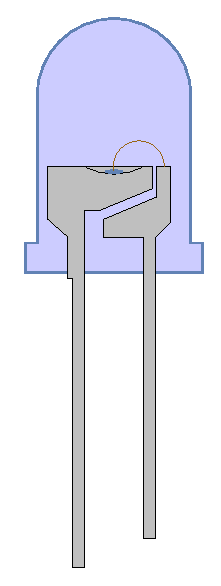
\includegraphics{Anhang/Tikz/ledFkt.pdf}};
  % Marks 
  \node[] at (2.7,6) {\tikzmark{lens}};
  \node[] at (2.8,4) {\tikzmark{wire}};
  \node[] at (2.05,3.4) {\tikzmark{crystal}};
  \node[] at (2.6,0.5) {\tikzmark{anode}};
  \node[] at (1.4,-0.5) {\tikzmark{cathode}};
  cathode
\end{tikzpicture}

\columnbreak
\vfill\null 
\begin{itemize}
  \itemsep20pt
    \item[] \tikzmarkcomment{item1}{Gehäuse das als Linse dient aus Epoxidharz}
    \item[] \tikzmarkcomment{item2}{Anschlussdraht für den Halbleiterkristall aus Gold}
    \item[] \tikzmarkcomment{item3}{Halbleiterkristall in Reflektorwanne}
    \item[] \tikzmarkcomment{item4}{Anode der LED (Langer PIN)}
    \item[] \tikzmarkcomment{item5}{Kathode der LED (Kurzer PIN)}
 \end{itemize}
\vfill \null

\begin{tikzpicture}[remember picture,overlay]
  \path[red, thick,-] (lens.east) edge [out=0 , in=180] (item1);
  \path[red, thick,-] (wire.east) edge [out=0 , in=180] (item2);
  \path[red, thick,-] (crystal.east) edge [out=0 , in=180] (item3);
  \path[red, thick,-] (anode.east) edge [out=0 , in=180] (item4);
  \path[red, thick,-] (cathode.east) edge [out=0 , in=180] (item5);
\end{tikzpicture}
\end{multicols}

\subsection{Vorwiderstand einer LED berechenen}


\section{Schaltungsentwicklung mit Fritzing}


\chapter{Hintergrundwissen: Free Software Foundation and Creative Commons}

\section{Open Source und Creative Commons}



